%!TEX root = ../Masterthesis.tex
\chapter{System conception}\section{Technical conception}
\begin{figure}[H]
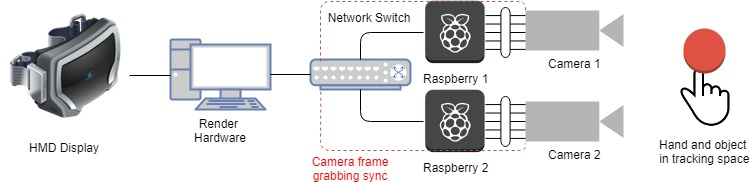
\includegraphics[width=\textwidth]{images/technical_setup.jpg}
\caption{Technical conception of the single hardware parts}
\label{fig:technical-copnception}
\end{figure} 
\todo{edit fgure above}As depicted in Figure \ref{fig:technical-copnception}, the technical components of the setup are realtively simple.Instead of using one large dimensioned unit which takes care of all calculations, the image processing steps that have to be done on both stereo images anyway, are outsourced onto the Raspberry Pi's.
The image processing can be done on the two Pi's in parallel, which cuts down processing time. Furthermore the image data stay on the device and does not have to be sent to a min unit whch would introduce network and data reading latency.\\
The two \textbf{Raspberry Pi 3 Model B}, which are used as the controllers for the \textbf{Raspberry Pi Camera} are connected via network cable to a network switch. A connection over wireless network would be possible with the on-board capabilities, but this might create latency problems and/or signal interference with other existing networks. Therefor a cable connection is the safer solution.
The switch also connects to the "Master" PC to which the "Slave" Pi's communicate their data. The Master also takes care of the stereoscopic calculations,as it is dimensioned with far more computational power than the slaves. The 2D positional data from the slaves and the calculation results from the stereo image disparity is fed into the hand model running on the "Master". The model solution is then applied to the digital hand model and rendered.
\newpage
\section{Construction Details}
For the physical construction of the system, it is important to know what the primary use case of the system will be. A mobile system is principally not impossible as the Raspberry Pi's could be run with battery power. A wireless communication leads to the beforehand described Problems and a long enough cable connection is rather cumbersome. Furthermore the cameras need to be calibrated at a fixed position for correct depth measurements. Some kind of mounting harness would be needed where the cameras stay in a fixed position.\\
A much easier approach for the first prototype is defining a seated usecase for the user. Since the systems main chore is to track the hand of the user, a seated position reduces position tracking errors as one does not have to take account large positional changes of the rest of the body.
The tracking volume that needs to be accomplished for a seated position is also reduced by our physical limitations of the arm length. A tracking volume of about $100x100x100$ cm should be sufficient to track most of the movement.\\
A frame of 30x30 mm construction Profile is used as base to mount all the components of the system. To reduce posiible color reflections from the background of the tracking space, black fabric is used as background material. The other components of the system are:
\begin{itemize}
\item 2 Raspberry Pi 3 Model 3 with 1GB RAM and a 64GB microSD Card running a current Raspbian OS and a C++14 compiler
\item Compiled version of OpenCV and Boost librarys
\item 2 Raspberry Pi Camera Modules V2 with a 100 cm connector cable
\item Ethernet Switch
\item Monitor for calibration and debugging of the Raspberry side software
\item PC capable of supporting a HMD and a current Java version 8+
\item Mounting peripherals
\item Active cooled case for the Raspberry to help with heart reduction
\item Two micro USB power supplies with 3.0 A output current
\end{itemize}
The active cooled Raspberry pi cases are an optional part of the construction, but the real time image processing on the CPU of the Raspberry together with the running camera produces larger amounts of heat than in normal operation mode.The applied heat sinks and the active cooling fan help with faster heat dissipation. The 3.0A power supply units are recommended as lower output currents still work but can lead to a power brown out on the system. This can cause system damage over longer usage times and even make the used SD card unreadable.
\subsubsection{Mounting peripherals}
The used cameras are basically the camera sensors mounted on a pcb with an optic. They have 4 drilling holes as fixations points. A simple holder plate was constructed digitally and printed with a 3D Printer for faster prototyping. The holder was designed as two parts to be able to change the mounting distance of the camera setup from the construction profile if needed. The two parts are held together by 4 screws for permanent fixation. Cut outs in the mounting plate for the cameras provide the ability to mount the cameras with two machine screws and move to end position of the cameras along a fixed axis (see Figure \ref{img:camera_holder}). This ensures that the cameras are mounted on one axis. It furthermore give the opportunity to change the interaxial distance of the cameras if needed. for the current setup this distance will be set to 75 mm which corresponds to the interaxial distance of the human eyes.
\begin{figure}[H]
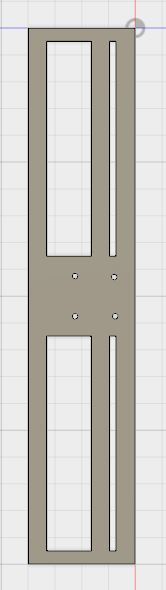
\includegraphics[height=\textwidth, angle=90]{images/CAmera_holder_2.JPG}
\caption{Technical drawing of the camera holder}
\label{img:camera_holder} 
\end{figure}
\begin{figure}[H]
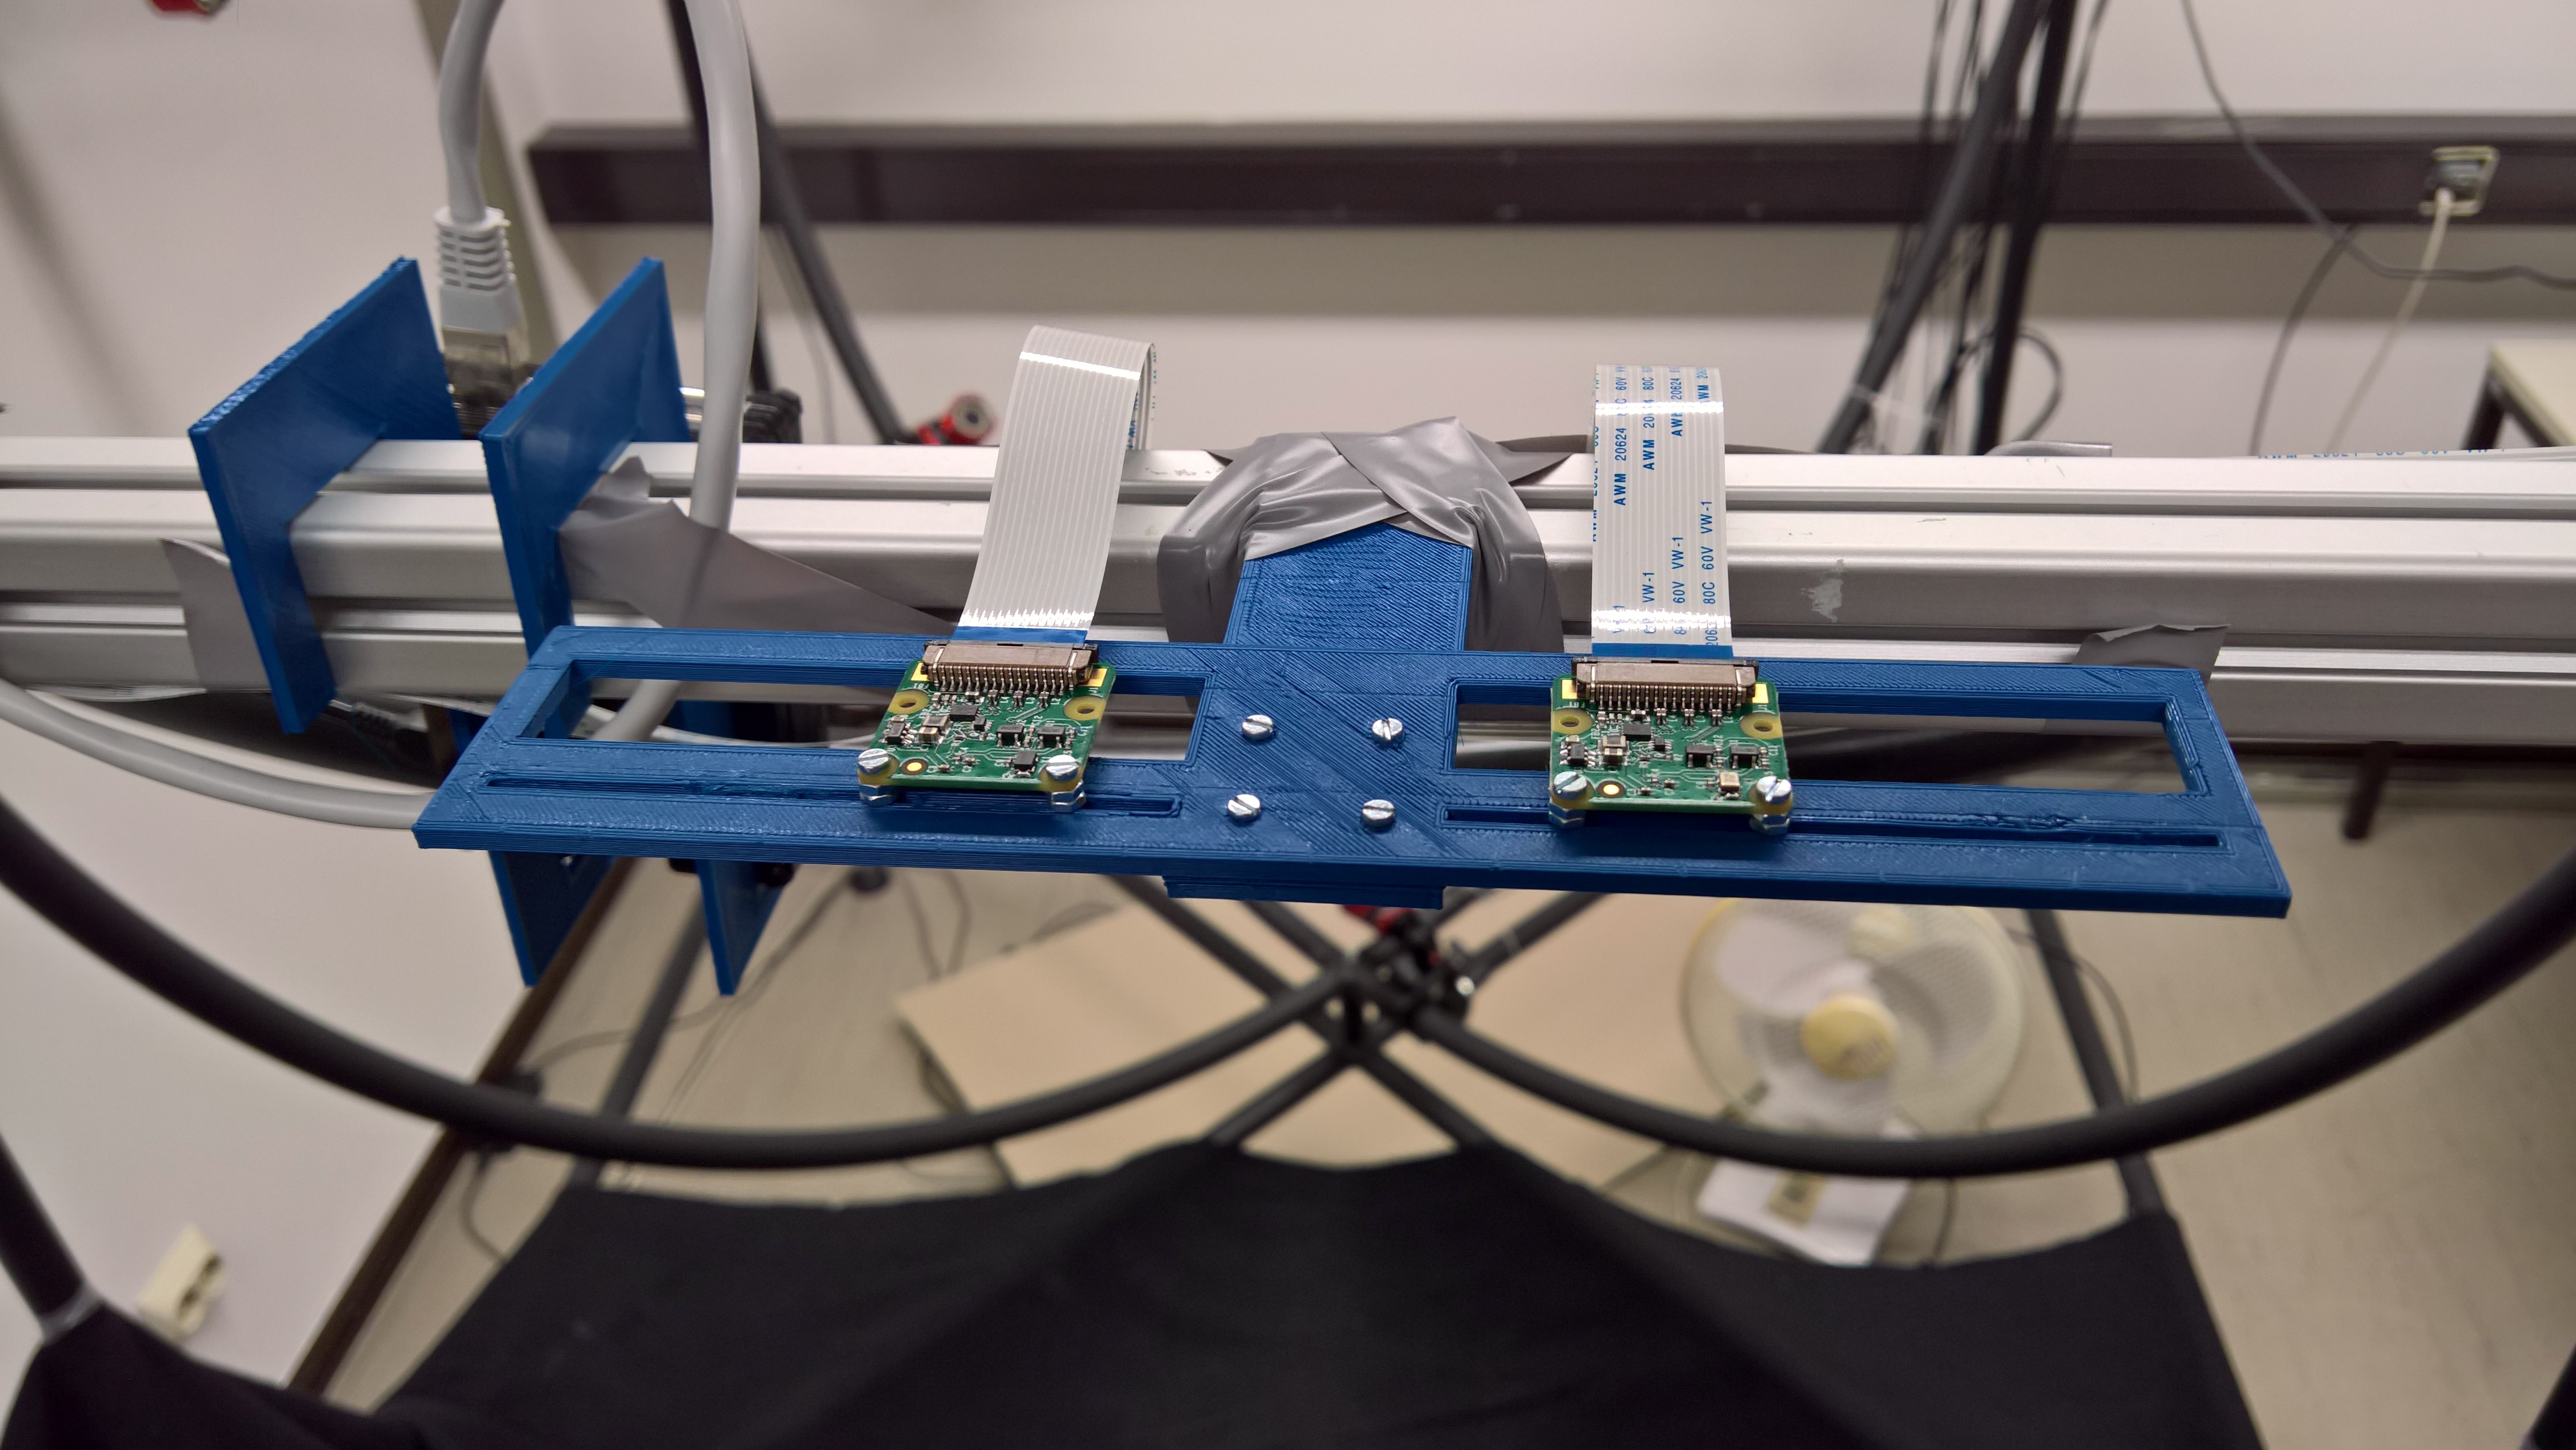
\includegraphics[width=\textwidth]{images/real_camera_setup.jpg}
\caption{Printed camera holder with mounted cameras}
\label{img:camera_real} 
\end{figure}
\section{Image analysis on the Raspberry}
For the image analysis part, \textit{OpenCV3} with it's \textit{Python 3} bindings is chosen. The \textit{OpenCV} package needs to be downloaded and compiled onto each device before it can be used.
Before the actual image analysis part can take place, the used cameras need to be calibrated. As they are basically pinhole cameras, they introduce amounts of radial and tangential distortion to the images. These distortions need to be compensated for, especially when using them as source for the stereo images. Image distortion in these pictures would lead to incorrect calculations for image depth.
\textit{OpenCV} supplies the tools to calculate the distortion parameters as well as the camera matrix \cite{Opencv.2018}.
The camera matrix is basically a description for the transformation of points in 3D object space to the 2D image space of the camera. For the used Cameras, we can consider a central projection of points in space onto our image plane. The center of the camera is considered the center of an euclidean coordinate system and the projection plane \textbf{z} is located at distance \textit{f} equal to the focal length of the camera.
\todo{read and reformat}
\begin{figure}[H]
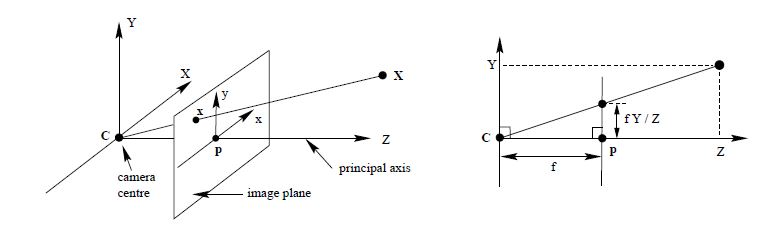
\includegraphics[width=\textwidth]{images/pionhole.JPG}
\caption{Image point projection for pinhole camera systems\cite{Hartley.2000}}
\label{pinholecamera_mapping} 
\end{figure}
As shown in Figure \ref{pinholecamera_mapping}, a point from the object space can be projected onto the image plane by drawing a ray from the object space point to the camera center. The intersection point of the ray with the image plane defines the projection point. With this knowledge the projection can be described as :
\begin{equation}
(X,Y,Z)^{T} \mapsto (fX/Z,fY/Z)^{T}
\end{equation}
\todo {elaborate}
For the calculation of the image distortion , \textit{OpenCV} uses a chessboard image for calibration. The printed image is held in front of the camera at a constant distance and rotated and positioned differently. After every position/rotation change an image of the pattern should be taken.
These images are then used to find the corners at the intersection of the black and white squares. With the previous knowledge of the square sizes, the projection errors in radial and tangential directions can be calculated:\todo{add Source code}
\begin{equation}
\begin{split}
x_{tanDistorted}&=x(1+k_{1}r^{2}+k_{2}r^{4}+k_{3}+r^{6})\\
y_{tanDistorted}&=y(1+k_{1}r^{2}+k_{2}r^{4}+k_{3}+r^{6})\\
\\
x_{radDistorted}&=x+[2p_{1}xy+p_{2}(r^{2}+2x^{2})]\\
y_{radDistorted}&=x+[p_{1}(r^{2}+2y^{2})+2p_{2}xy]\\
\end{split}
\end{equation} 
As can bee seen from the above equations, the parameters that need to be calculated are $k_{1},k_{2},p_{1},p_{2},k_{3}$.
\todo{continue}

The python program prototype that is used for tracking the specified color markers is comprised of the following components:
\begin{itemize}
\item Image acquisition from camera
\item Image conversion to HSV colorspace
\item Mask construction and filtering
\item Contour finding an position calculation
\item Sending of positional data via network as UPD package
\end{itemize}
\subsection{Image acquisition from camera}
As the computation times for image filtering and mask generation may vary, it makes sense to separate the image acquisition from the computation part.Therefore the loading of the image data frame from the camera is outsourced into its own thread.The synchronicity of the two frame reading threads is assumed for the first implementation and has to be tested on a finished setup.
\\
The tread takes the data of the current image frame and hands it over to the main thread, where the image processing is handled. For the first frames, the full image data is needed as the position of the markers is not yet known. Performance-wise, this introduces a lot of overhead, since each mask generation step for the specific colors hast to go through the complete image data, meaning every pixel has to be read out at least 5 times to get the tracking for all different markers.
\begin{figure}[H]
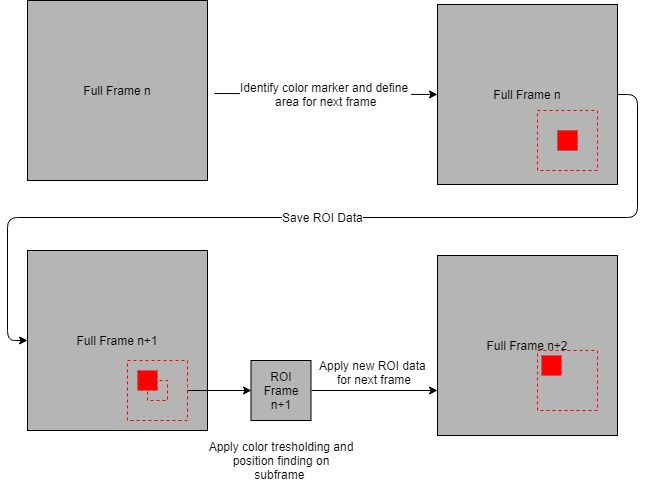
\includegraphics[width=\textwidth]{images/ROI.jpg}
\caption{ROI calculation for consecutive frames}
\label{roi_calc} 
\end{figure}
After a few frames, we get hold of the marker position and can define a reduced region of interest (ROI) on the image (Figure \ref{roi_calc}). The new ROI results from the positional data of the previous frame and has to be dimensioned correctly as to incorporate the possibility of large position differences between consecutive frames.
Furthermore the offset position, preferably the top left corner of the region, has to be kept track of. By taking a sub-region of the frame as input for further processing, the resulting coordinates relate to the top left corner of this sub-region as origin. Consequently only the first set of coordinates has the correct origin as reference point for the next frame. Consecutive frames need this information to retrieve the correct sub-region from the full frame by adding the offset to the calculated positional data.
First frame ROI calculation is based on a minimum axis-aligned bounding box(AABB) fitted onto the marker. The offset value for the ROI is added to the bounding box values resulting in a rectangle data-set containing the position of the offset top-left corner $\vec{\mathbf{tl}}$ and the offset 
\textbf{width} and \textbf{height} of the ROI rectangle:
\begin{equation}
\begin{split}
\vec{\mathbf{tl_{0}}}&=(AABB_{x_{0}}-\text{offset}_{x},AABB_{y_{0}}-\text{offset}_{y})\\
\mathbf{width}&=AABB{w_{0}}+(2\cdot\text{offset}_{x})\\
\mathbf{height}&=AABB_{h_{0}}+(2\cdot\text{offset}_{y})\\
\end{split}
\end{equation}
These values are taken to extract the sub-region of the consecutive at $\vec{\mathbf{tl}}$ with size of width and height. The $\vec{\mathbf{tl}}$ value is also saved as offset value $\vec{\mathbf{OffPos}}$ .
The position calculation for the proximate frame will utilize the offset value as follows:
\begin{equation}
\begin{split}
\vec{\mathbf{tl_{1}}_{x}}&=x_{1}+\vec{\mathbf{OffPos}}_{x}-\text{offset}_{x} \\ \vec{\mathbf{tl_{1}}_{y}}&=y_{1}+\vec{\mathbf{OffPos}}_{y}-\text{offset}_{y}\\
\mathbf{width}&=AABB_{w_{1}}+(2\cdot\text{offset}_{x})\\
\mathbf{height}&=AABB_{h_{1}}+(2\cdot\text{offset}_{y})\\
\end{split}
\end{equation}
This should result in the correct positional data for all frames following the initial frame.
Finally,the resulting rectangle has to be fitted onto the size boundaries of the full image frame. When applying a fixed offset value, the resulting region that will be extracted from the following frame might reach outside the size boundaries of the full frame. This can happen when the markers are positioned near the edges of the frame. Trying to read out pixels outside the available size of the image will without doubt result into an error by reason of unavailable data at these points. Therefore the combination of position width, height and offset has to be clamped to fit into the available image data:
\begin{equation}
\begin{split}
\textbf{width}&=\text(max(0,min(\mathbf{width},image_{width}))\\
\textbf{height}&=\text(max(0,min(\mathbf{height},image_{height}))
\end{split}
\end{equation}
Another option which could be evaluated instead of clamping the area would be shifting the offset point to a position where it does not violate the image boundaries and  thereby preserving the size of the ROI.
Should no marker be found in the defined ROI or the certainty of the result is not high enough, the frame has to be dropped and the next frame should utilize the whole image data.
\subsection{Image conversion to HSV colorspace}
The image data that is supplied by the camera comes in an RGB data format, which we could already use for the further calculation. It does though make more sense to convert the input data into the HSV colorspace. Since we are not using high precision cameras, it is necessary to define a range of color values around the desired color which we want to track. The HSV colorspace is displayed as a cone, in comparison to the RGB colorspace, which is displayed as a cube. The color values for the HSV space are all located on a circle spanning form 0 to 360 degrees. The Hue value (H)corresponds to the angle on the circle, where $0^\circ$ corresponds to a reddish color, $120^\circ$ lies in the area of green and $240^\circ$ and above correspond to blue. The saturation value (s) corresponds to the amount of white the color contains  where 0 is pure white and 100 corresponds to the fully saturated color. For optimal results, only highly saturated colors should be used to ensure correct color detection. The last component is the value component (V) which describes the intensity of the color. Alike the value settings for the saturation, value ranges of at leas 50 should be used for tracking precision.
For tracking the five fingers of the hand we need five distinguishable colors. Here the primary colors red, green and blue will be the choice for the first three colors. The other two selected colors are orange and yellow. To be able to clearly distinguish these colors in the video frame, a constant and homogeneous lighting is needed as well as a color temperature of the lighting that is in the neutral area to not change the color of the markers.
\\The color conversion from the input RGB values to the desired HSV colorspace is done as follows:
\begin{equation}
\begin{split}
hsv_{low}&=(hue_{targetcolor}-sensitivity,100,100)\\
hsv_{up}&=(hue_{targetcolor}-sensitivity,100,100)\\
\end{split}
\end{equation}
\subsection{Mask construction and filtering}
\todo {orig image and mask images for display}
These values are the used as the parameters for a mask generation which generates a binary mask for the current frame where all pixels whose values lie outside of the specified range are set to zero (black) and the remaining are set to 255 (white).For these masks to work properly, any other larger objects that might contain similar colors should be removed from the scene to eliminate wrong tracking data. The used cameras run on an automated white balance and exposure mode. The variation of these values can cause shifts in the appearance of the colored markers and therefore alter the generated masks. To compensate for white balance shifting, a non-white ideally diffuse reflecting background should be used for the tracking space. Also the auto modes should be turned off and appropriate values for white balance and exposure have to be determined at the initialization step of the system.As all digital cameras tend to have signal noise in the sensor data , high frequency  noise in the color channels will be present. This noise should be filtered out before any further computation on the image data can be done.
The first step in this progress is to use a Gaussian filter to blur the mask.\\
The Gaussian filter acts as a low pass filter for the image. The application of the filter cuts out high frequency noise generated by the sensor electronic and other factors. The downside of applying a Blur onto the generated image is a loss of detail. As the markers will not be utilizing complex geometric forms or fine patterns, the loss of details is acceptable.\\
After this step an erosion and a dilation is applied to the image tho further eliminate unwanted noise. A combination of these two morphological operation is used to further improve the data of the thresholded binary image\cite[chapter~3.11-12]{Davies.2017}.
Erosion and dilation operation on thresholded images perform the tasks of removing light spots on dark backgrounds as well as dark spots on light backgrounds. These spots are usually the result of the remaining image noise after the blurring or incorrect pixel values from the camera which case the pixel to be incorrectly thresholded.
To apply the specific operators to the image a mask ( often also called kernel) needs to be defined. These masks normally consist of an n x n shaped matrix where the values in the matrix rows and columns are either one or zero for binary images. An odd number of rows and columns is usually used to be able to define a center pixel. The central entry of the matrix corresponds to the current pixel of the image for which the morphological operation is to be applied. As the data of the pixel should be preserved, the value is set to one. 
\begin{figure}[H]
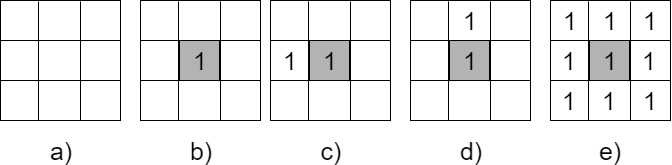
\includegraphics[width=\textwidth]{images/morpological_kernels.jpg}
\caption{ Example Mask of 3x3 size :\textbf{a)} empty mask \textbf{b)} Mask that keeps pixel value  \textbf{c)} combination of b) with a left shift   \textbf{d)} combination of b) with an upshift   \textbf{e)} isotropic mask}
\label{morphological_ops} 
\end{figure}
The processing of these matrices is not very complex. The central pixel value and the values of the neighboring pixels are taken and summed up.The ones in the matrix outside of the center value define if the pixel is taken in for the operation. A threshold value is then defined. The result of the sum operation is compared to the threshold value. If above the threshold, the central pixel value is altered, depending on the image operation. If below, the current value is kept.
\begin{algorithm}
\SetAlgoLined
\SetKwInOut{Input}{input}
\SetKwData{Threshold}{threshVal}
\SetKwData{Result}{result}
\SetKwData{CentVal}{centVal}
\SetKwData{OpVal}{opVal}
\Input{threshold $threshVal$ value for the calculation, image segment $imgSegment$ of size $n\times n$, mask $morphMask$ of size $n \times n$, operation value (0 or 1) $opVal$, value of central pixel $centVal$}
\BlankLine
\KwResult{New value for pixel}
\BlankLine
\For{$i\leftarrow 0$ \KwTo maskHeight}{
	\For{$j\leftarrow 0$ \KwTo maskWidth}
	{
	 \If{$morphMask[i,j] = 1$}{\Result$\leftarrow$\Result$ +morphMask[i,j]$}
	}
}
\If{\Result $>=$ \Threshold}{\CentVal$=$ \OpVal}
\caption{Pseudocode for the the pixel value calcuation}
\label{mask_calc_pseudocode}
\end{algorithm}

When using for example the isotropic matrix displayed in Figure \ref{morphological_ops} e) and setting a threshold of 8 on an dilation operation, the result would be the filling of a white pixel when surrounded by black pixel. The same operation on an erosion would lead to an removal of a black pixel surrounded by white pixels.

The combination of the morphological operator erode and dilate leads to two methods called \textit{morphological opening} and \textit{morphological closing}. The idea behind these two is to use the two basic operation in a certain order to enhance the binary image quality \cite[chapter~3.12]{Davies.2017}.
The formal definition for the operation:
\begin{equation}
 \begin{split}
O&=Original\; image \\
\oplus&= Dilation\; operation\\
E&=Erosion\; mask\\
\ominus&= Erosion\; operation\\
D&=Dilation\; mask\\
\circ&= Morphologic\; opening\\
\bullet&= Morphologic\; closing\\
\\
O\bullet D&=(O\oplus D)\ominus E\\
O\circ D&=(O \ominus E)\oplus D\\
\end{split}
\end{equation}

The \textit{morphological closing} operation is applied first to eliminate so called "salt noise" (white pixels in black area), narrow cracks, channels and 	small holes in the original image. The major part of the work for this operation is done on the areas where not tracking marker is found. It removes the remaining noise left over from the blur or signal distortion.

The application of the \textit{morphological opening} removes so called "pepper noise", fine hairs and small protrusions. 
The outcome of the practical application of the opening is the removal of wrong pixels inside the area of the color marker in the image. This helps with the later calculation of the bounding boxes as the algorithm searches for the largest closed area int the image.
Generally the closing of an image enlarges it while filling bright defects inside of an black area and the opening makes it smaller while removing bright defects on a dark surface.
As the system will not be handling large image data, the mask sizes can be kept low, utilizing the above described $3\times 3$ mask size. The structure options provided by \textit{OpenCV} contain a cross structure, an elliptical structure and a isotropic version. As it would be useful to get all surrounding image data and the tracking markers will not have complex geometric structures, the isotropic mask structure should be sufficient. The threshold limit  should be set to an  initially reasonable value with further testing on the running setup.
\subsection{Contour finding and position calculation}
With the cleaned mask we can continue and search for the white areas in the mask which might represent our target. Under the assumption that we have removed all other parasitic objects from the image, the marker should be the largest area of positive pixels in the mask frame. Therefore only the largest area found in the search is taken as the desired tracking marker. For the selected area, a fitting bounding box is calculated and the center of this box is used as the positional parameter of the tracking marker.
\subsection{object tracking}
\todo{add object tracking method -> visual or HTC vive tracker}
\section{Systems communication}
The data that is generated on the two Raspberry's has to be communicated to the "parent" unit where further processing is done. The data delay between the different endpoints should be minimal. As the data is streamed in real time, protocols like TCP, which utilize control mechanisms for package order and receiving of data use to much overhead. In the time frame needed for the protocol to request a missing package again, the data will already be obsolete. \\Furthermore, the amount of data that is send in each data frame is minimal, as this is only the position value of the specified number of tracking points and some separators for string processing. Since the devices will be connected to a local network via a switch, network workload from other devices ans protocols can be assumed as minimal and not impacting transport time.\\
Regarding all these points a simple UPD protocol setup seems to be the best choice. Package loss that might appear with UDP is not critical as it means only the loss of one frame Data set.\\
It has to be ensured that the UDP data streams from both devices are recorded separately to ensure that the data can be separated correctly for the stereoscopic calculations.
The possibility to send multi- and/or broadcast messages via UDP also open up an easy way of communication between the "parent" and the Pi's for control communication.
\begin{figure}[H]
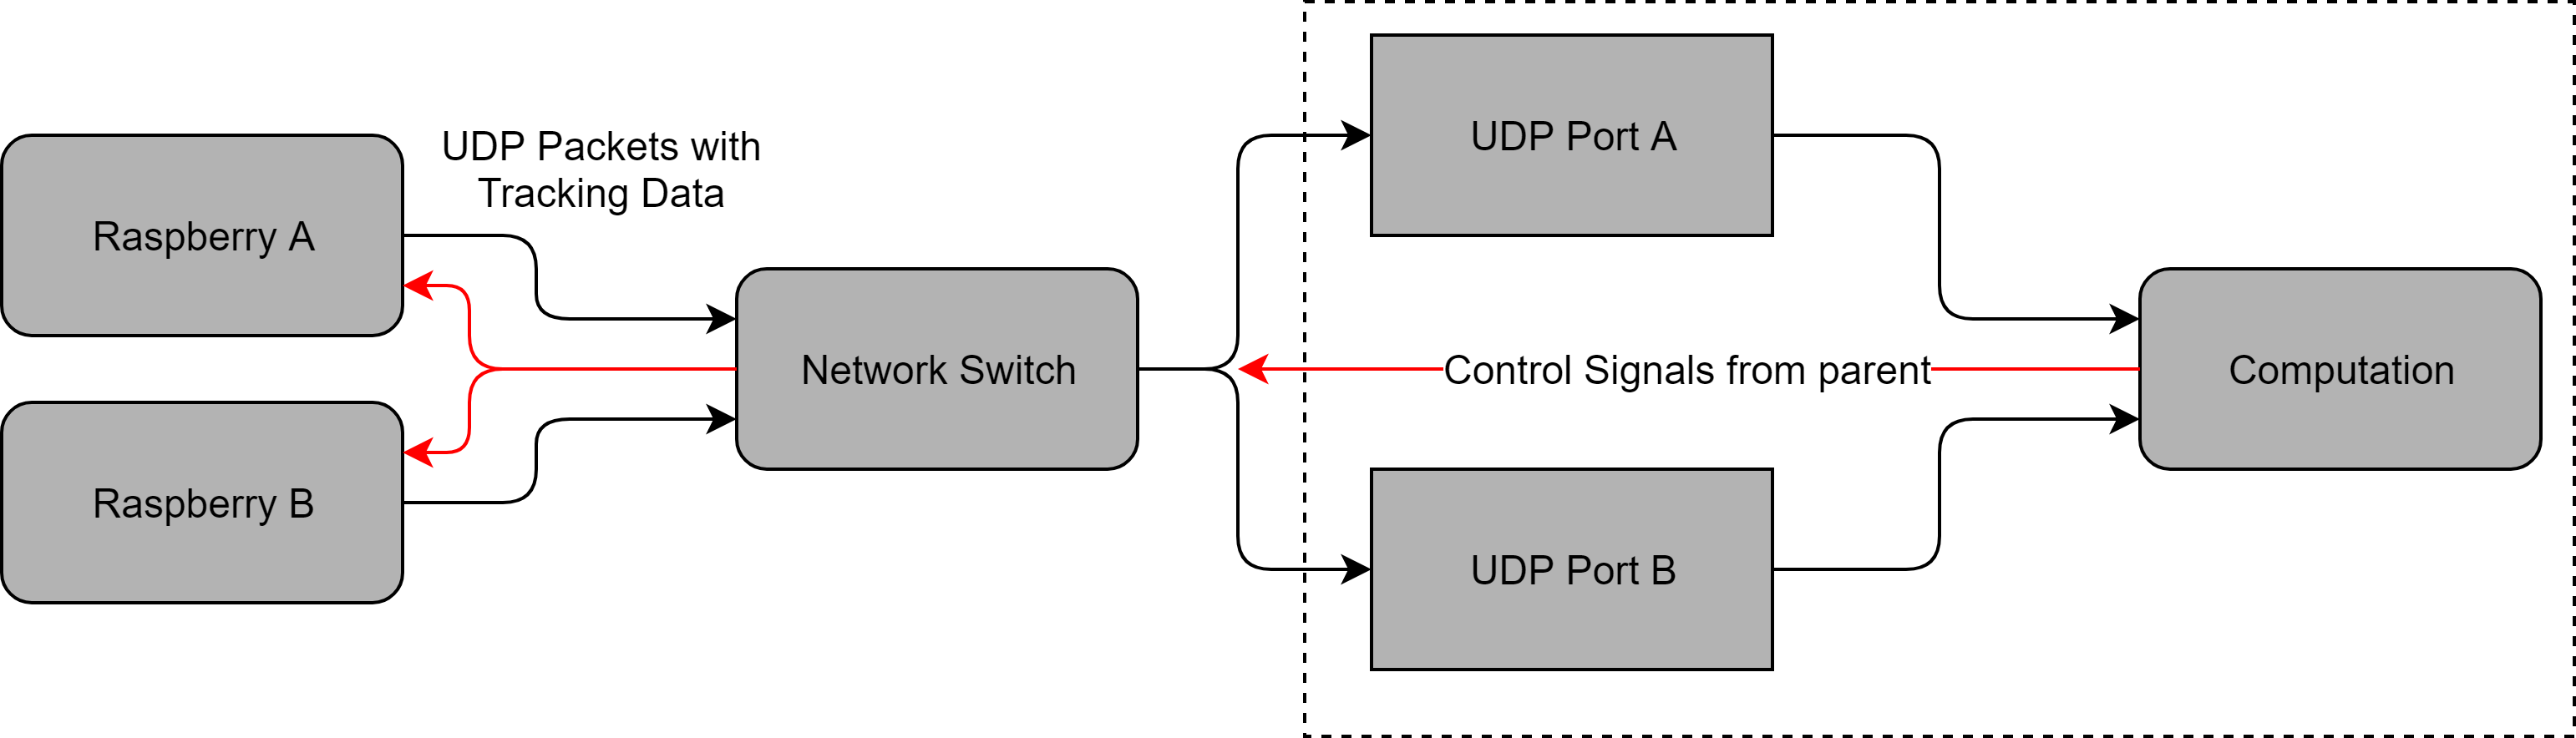
\includegraphics[width=\textwidth]{images/Network_Diagram.png}
\caption{Workflow for the UDP Data packages that are send from the Raspberrys to the parent PC}
\label{img:netzwerk_diagram} 
\end{figure}
\newpage
\section{Data processing on the receiver side}
\begin{wrapfigure}[26]{r}{\textwidth/2}
\label{img:hand_model_workflow}
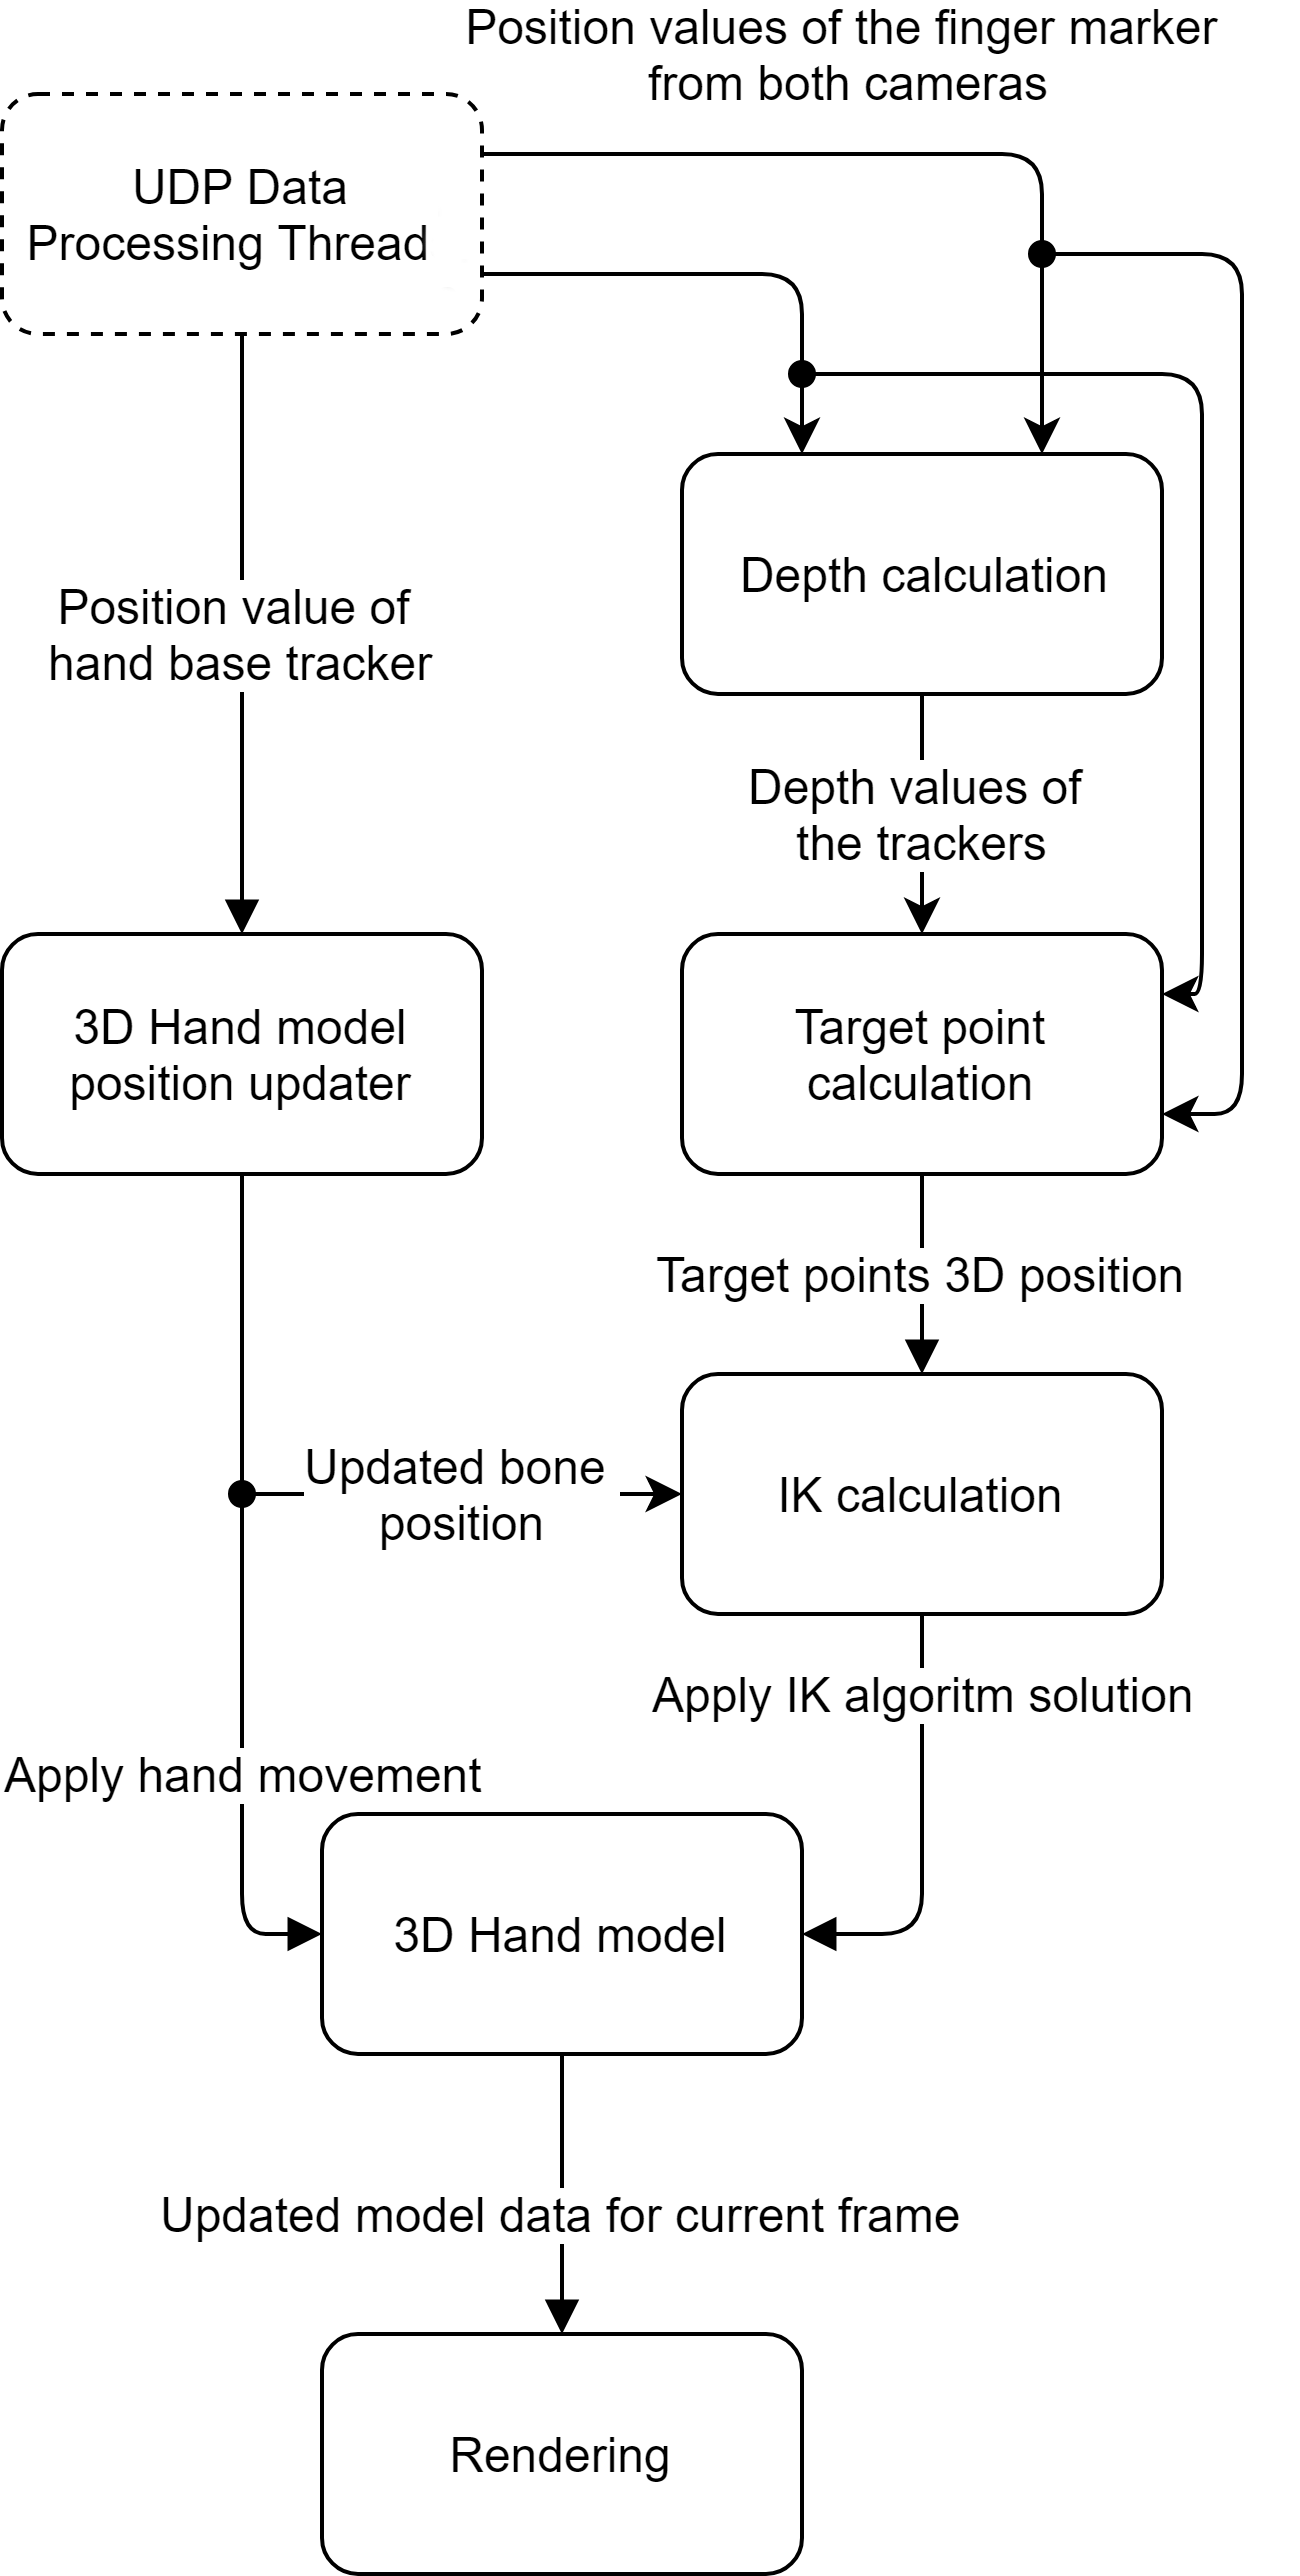
\includegraphics[width=\textwidth/2]{images/Rendering_workflow.png} 
\caption{Overview diagram of the processing steps for the hand model data on the client side}
\end{wrapfigure}
The parent unit receives the two UDP data streams form the Raspberry's. To ensure that the two data streams are separated and therefore distinguishable, each stream receives a dedicated listening port on the client side(Figure \ref{img:netzwerk_diagram}). This separation of data streams also makes it possible to separate the UDP listeners to separate running threads in the background, taking away the task of data processing from the main thread which is already tasked with the rendering of the virtual scene. The positional data will be encoded as comma separated x and y coordinate set. Data separation is done by a simple semicolon as a separator between the coordinate sets. This takes very simple substring operations on the client side to extract the single coordinate sets form the string that is send with the UDP package.
After the string decoding, the extracted values are written into thread-safe variables.This allows the system to read current data without conflicting the writing process of the UPD threads.
\subsection{Stereoscopic calculations}
The positional data that is extracted in the UDP data processing only consists of 2D position data of the tracked marker on the image plane. To retrieve depth information for correct spatial placement of the marker the image disparity of the two cameras can be utilized to calculate the object distance from the cameras.\cite{Tauer.2010}\\
Before diving into the mathematical concepts, some essential terms have to be explained.
These are:
\begin{itemize}
\item Interaxial distance
\item Parallax
\item Zero-point plane
\end{itemize}
\subsubsection{Interaxial distance}
A stereoscopic imaging system is based off of our own human visual system as it produces stereoscopic images. Therefore such a system always consists of at leas two cameras which are mounted in parallel. The distance difference between the two cameras is called the "inter axial distance" of the system. The usual distance for such systems is the mean distance of the human eyes, which corresponds to around 75mm. Shifting the cameras closer together or further apart will change the resulting stereoscopic effect, where shifting the cameras closer together will enlarge objects and shifting the cameras further apart will make objects seem much smaller than they are. 
\subsubsection{Parallax}
Since the cameras are  separated by the \textit{interaxial distance}, a disparity in the generated images will occur. This means that the objects in the picture of the right camera will have a different position in terms of perspective than the images that result from the left camera. This resulting disparity is used to generate the 3D effect when displaying the images. The term "\textit{parallax}" is used to describe the comparison of the two images. The two images can have a negative, positive or zero \textit{parallax}.

\subsubsection{Zero-point plane}
The\textit{ zero point plane} is a special theoretical plane in a stereoscopic system. The location of the \textit{zero-point plane} defines the distance from the camera system at which the image points from both cameras match. Objects that lie before the \textit{zero-point plane} will have a negative \textit{parallax} and will appear closer to the viewer. Ton the opposite side, objects with positive \textit{parallax} will lie behind the zero point plane and therefore will appear further away.

\begin{figure}[H]
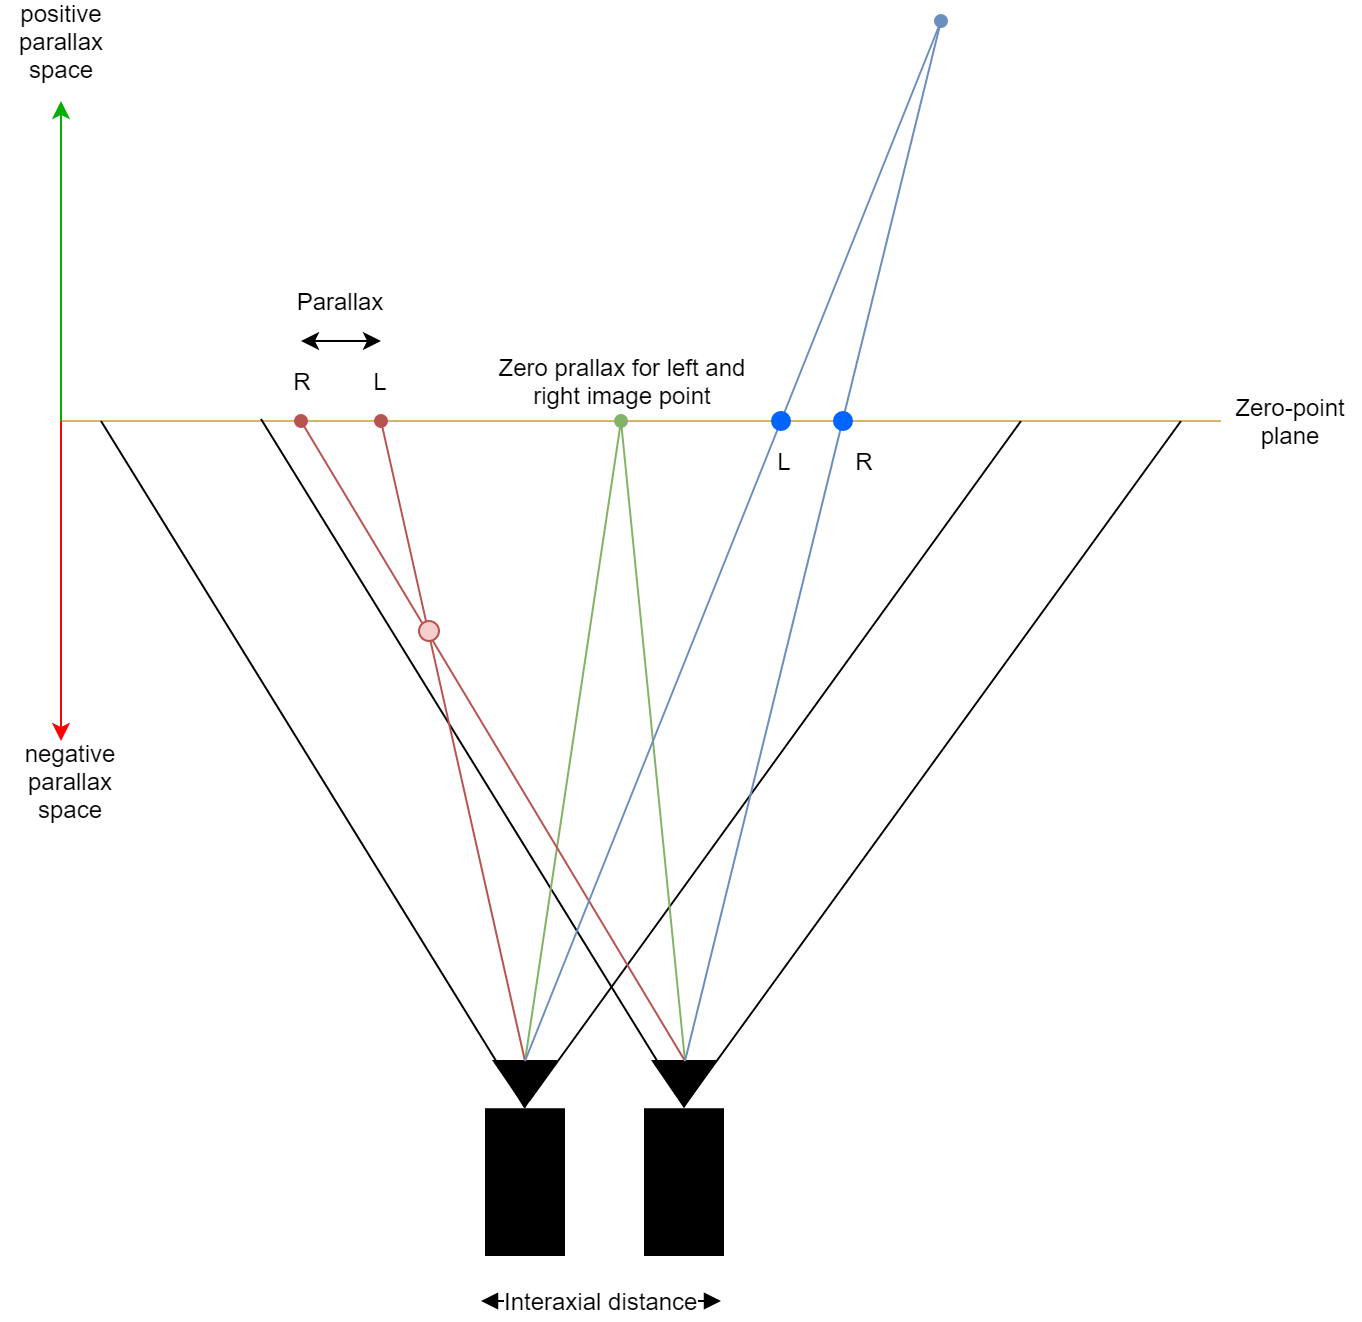
\includegraphics[width=\textwidth]{images/Stereo_diagram.png}
\caption{Stereoscopic areas}
\label{stereo_diagram} 
\end{figure}
Additional attention needs to be put in the camera setup before calculating depth form disparity. The cameras need to be checked for horizontal alignment to achieve correct values for the calculation.
\subsection{Depth calculation}
With correctly aligned system, one can calculate the distance of an object from the cameras using common trigonometric fundamentals\cite{JernejMrovlje.2008,YasirDawoodSalman.2017}.
\\
The position for the right camera will be denoted as $S_{r}$ and the position of the left camera will be denoted as $S_{l}$ (see Figure \ref{stereo_Dimmensions}a).The resulting distance of $S_{l}-S_{r}$ is the \textit{interaxial distance} $B$ of the system. The view angle $\theta$ of the Camera, which should be the same for both cameras, will respectively be $\theta_{1}$ and $\theta{2}$. From the camera positioning, the assumption of parallel optical axes is made. The angles of $\phi_{l},\phi_{r}$ describe the resulting angle between the optical axis of the camera and the object.
By using geometric derivations we can express that:\\
\begin{equation}
B= B_{1}+B_{2}=D\tan\varphi_{1}+D\tan\varphi_{2}
\end{equation}\\
Rearranging for D gives us:\\
\begin{equation}
D = \frac{B}{\tan\varphi_{1}+\tan\varphi_{2}}
\end{equation}
\begin{figure}[H]
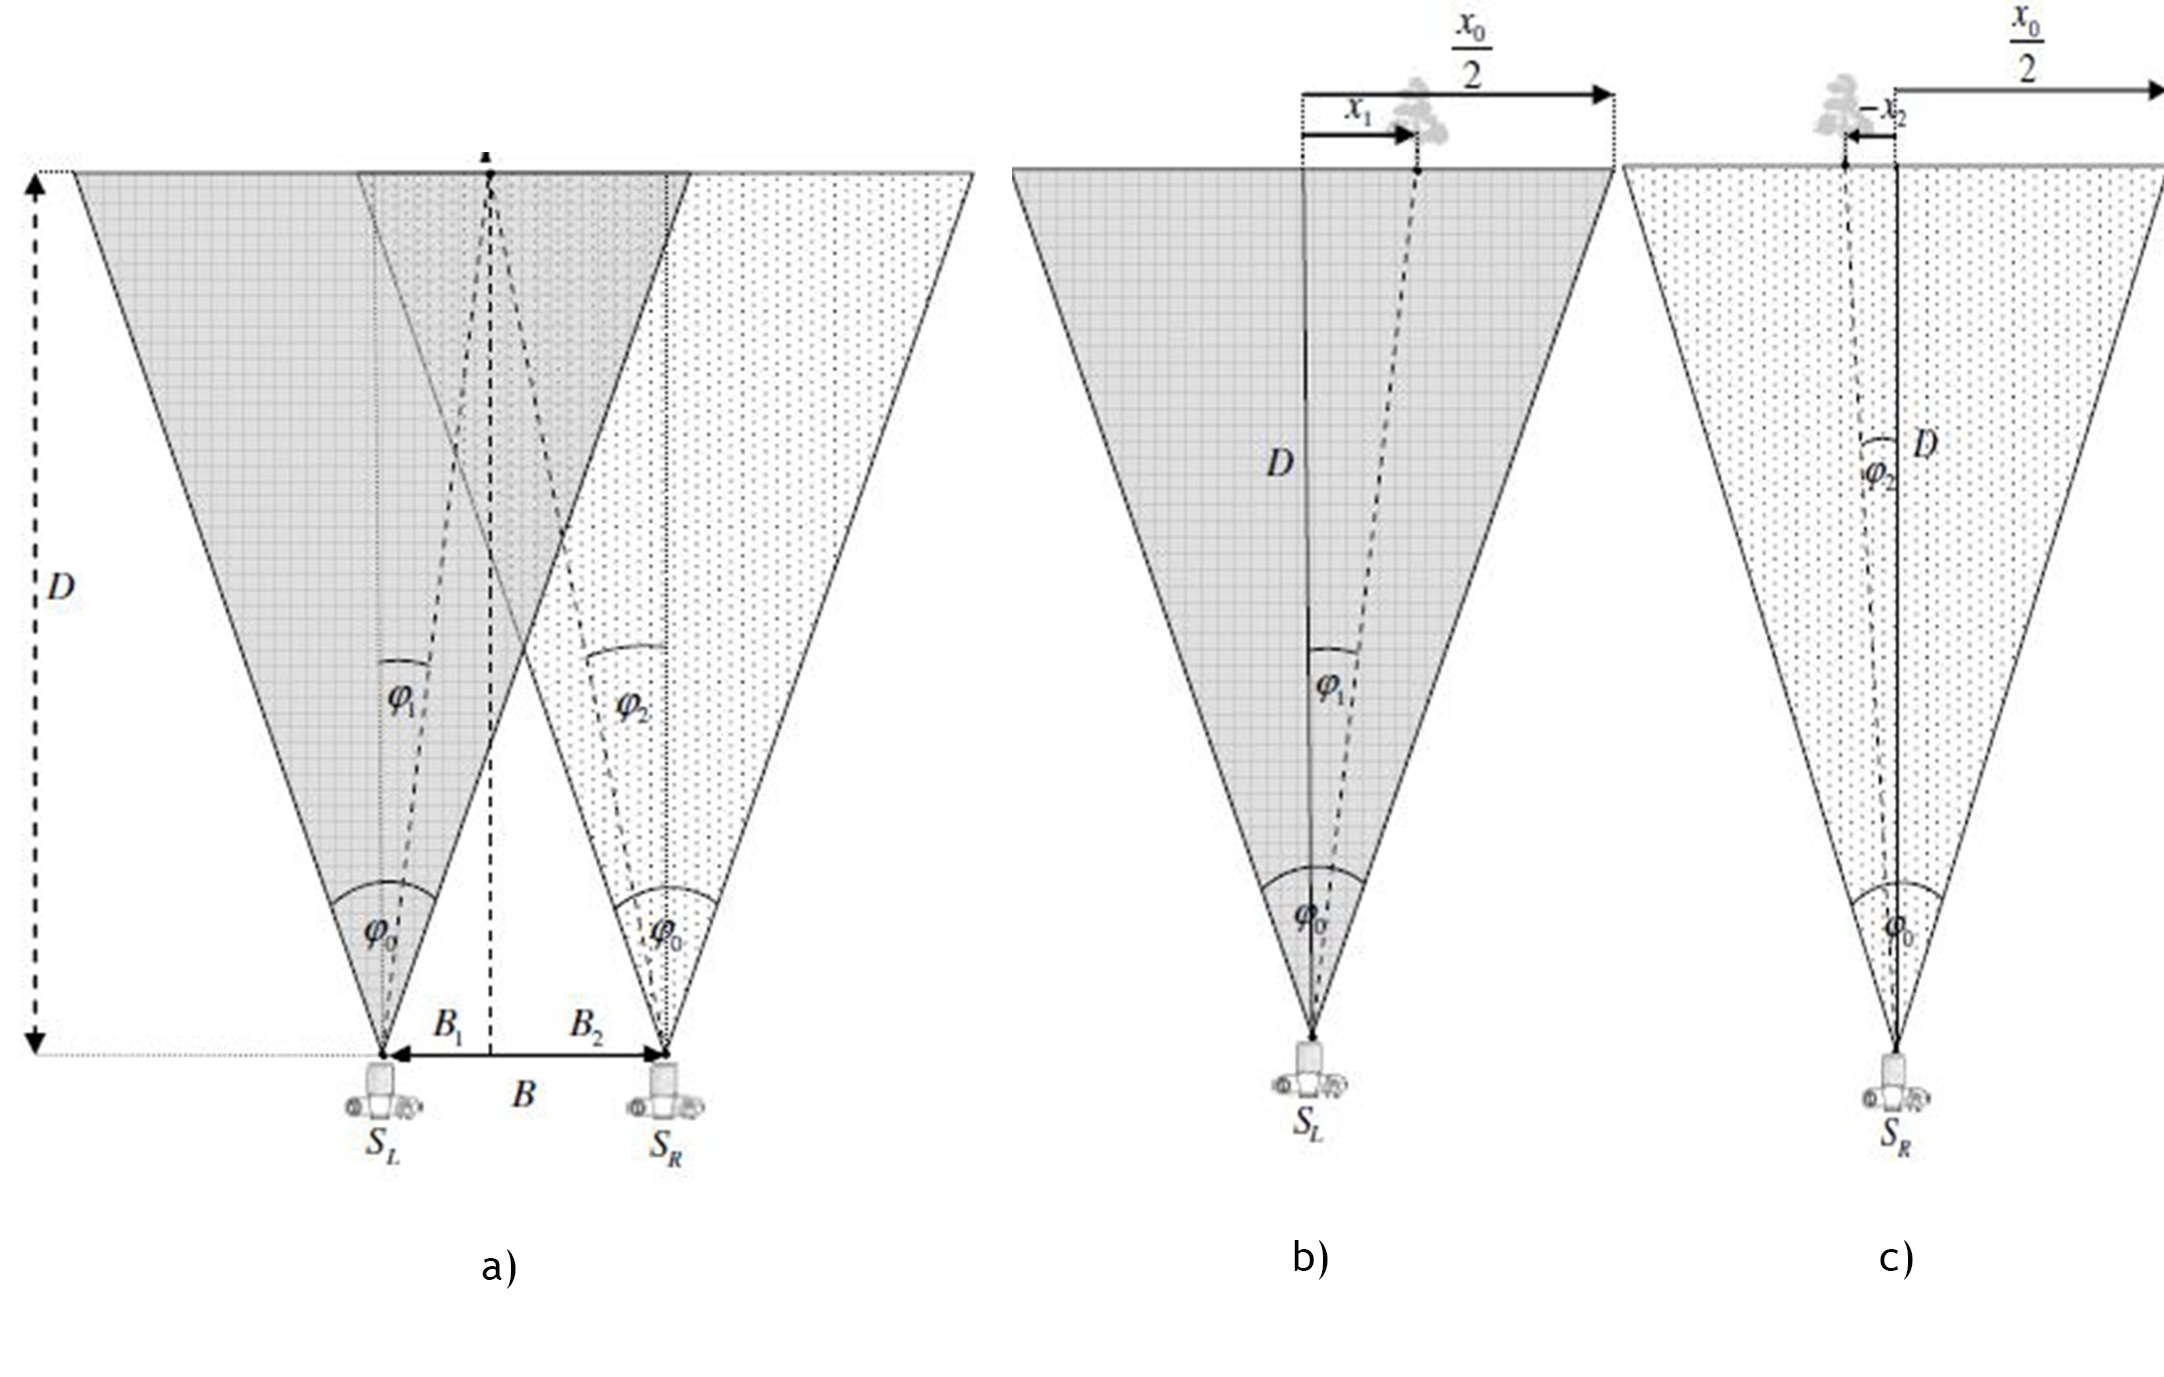
\includegraphics[width=\textwidth]{images/Stereo_Calc_4.JPG}
\caption{Dimmensions for calculation.Images from:\cite{JernejMrovlje.2008}}
\label{stereo_Dimmensions} 
\end{figure}
With Figure \ref{stereo_Dimmensions}b-c one can find that:
\begin{equation}
\frac{x_{1}}{\frac{x_{0}}{2}}=\frac{tan \varphi_1}{\tan(\frac{\varphi_{0}}{2})}
\end{equation}\\
\begin{equation}
\frac{-x_{2}}{\frac{x_{0}}{2}}=\frac{tan \varphi_2}{\tan(\frac{\varphi_{0}}{2})}
\end{equation}\\
Resulting in the calculation of D to be expressible as:

\begin{equation}
D=\frac{Bx_0}{2\tan(\frac{\varphi_0}{2})(X_{L}-X_{R})}
\end{equation}\\
Where B is the distance between the cameras,$x_0$ being the horizontal width of the picture format in pixels, $\varphi_0$ representing the viewing angle of the camera and $(X_{L}-X_{R})$ representing the disparity between the two images in Pixels.
\subsection{Model position update}
Before a solution with the inverse kinematics algorithm can be calculated, the hand movement in real space has to be matched with that on the digital side. TO achieve this, a further marker besides the finger markings is required. A sixth color marker has to be positioned at the connection point between hand and forearm to serve as a global position reference. The position and rotation difference between the last and current frame can then be calculated from the tracking values and then be applied to the whole model.
\subsection{Inverse Kinematics}

For the inverse kinematics calculation, the \textit{Fabrik} algorithm that is described in Section \ref{sec:fabrik_algorithm} was selected. It does not require complex matrix calculations and has a fast convergence rate. For the implementation of the algorithm on the client side, the \textit{Caliko} Java framework\cite{Lansley.2016} is used. There are also frameworks for other languages, but the java framework is platform independent. The library supplies all the needed classes and function tho create kinematic chains and structures as well as the implementation of the solving algorithm. It furthermore ships a visualization package which utilizes the Lightweight Java Game Library 3 (LWJG3).These classes can be used optionally for debug visualization or even as a base for a more sophisticated visualization as it is possible to load further components for i.e. VR into LWJGL.\\\\
For the inverse kinematics calculation to work properly the updated bone positions and the calculated target points from the finger tracking are needed.
For each finger a kinematic chain is set up with the correct bone length. The length of each bone has to be measured manually for the first prototype. Further iterations should provide a more elaborated and maybe even automated calibration procedure. The movement of each bone in the kinematic chains has to be restricted by constraints to restrict the algorithms solutions to physiological possible hand poses. The values for finger constraints that are described in Section \ref{sec:Physiological_structure_of_the_human_hand} should provide sufficient values. The resulting kinematic chains all have their own target point for which the algorithm can solve for. All chains will be grouped into a kinematic model for easier data handling. The kinematic model has a base and a connection structure through which the fingers are connected to it.  With this data, the algorithm is capable of calculating a solution for each kinematic finger chain and applying these values to the position. If the target is reachable, the digital finger position should match the pose of its real world counterpart.